\chapter{Statistical analysis}
\label{chapter:Statistics}

This chapter describes the statistical treatment that is used in the different analyses to make statements about the presence or absence of a particular process. The statistical tools and methodology used for searches at the LHC are described in detail.

\section{Hypothesis testing}
In particle physics the discovery or exclusion of a new physics model is performed through a statistical test. Two hypotheses, one describing the known physics processes, and one that in addition includes the new phenomena, are tested. The level of compatibility of the observed data with each of the two hypotheses is used to make a statement about the validity of the new physics model.
The two hypotheses are defined as follows:

    \begin{itemize}
    \item H$_0$ or Null Hypothesis: corresponds to the SM hypothesis.
      It is often referred to as the background-only (B) hypothesis.
    \item H$_1$ or Test Hypothesis: corresponds to the SM with the addition of a new signal process.
      For this reason, it is often referred to as the signal-plus-background (S+B) hypothesis.
    \end{itemize}
      In the search for the \ttH\ process, the SM without the Higgs sector is considered the background-only hypothesis, 
      while the signal-plus-background hypothesis includes the Higgs boson as signal. Searches for BSM signatures include the SM Higgs boson in the background model.

    The two hypotheses can be generalized by introducing a signal strength modifier, $\mu$, which acts as a multiplicative factor to the signal \xsec. The two hypotheses are recovered for $\mu = 0$, background-only hypothesis, and $\mu = 1$, signal-plus-background hypothesis.

    The compatibility of the observed data with a given hypothesis is quantified using a test statistic. From the test statistic a $p$-value can be computed, $p_\mu$, giving the probability that the observed data originates from a model with signal strength $\mu$. As a particular case, the $p_0$-value quantifies the agreement of the data with the background-only hypothesis.
    The $p$-value can be converted into the corresponding Gaussian significance, $Z$, defined as 
    the number of standard deviations that correspond to an upper-tail probability of $p_\mu$ for a Gaussian-distributed variable. 
    %It can be written as $Z=\Phi^{-1}(p_\mu)$, where $\Phi^{-1}$ is the quantile (inverse of the cumulative 
    %distribution) of the standard Gaussian distribution. 
    
    If a sufficiently low value of $p_\mu$ is found, it can be claimed that the tested hypothesis is false.\footnote{
    Unless the two hypotheses that are being tested are mutually exclusive, and the union of both covers all the spectrum of possibilities, the rejection of one hypothesis doesn't imply an affirmation of the second one.}
    The threshold to consider a probability low enough as to refute a hypothesis is arbitrary and a prescription has to be chosen.
    In particle physics, the convention has been adopted that a probability $p_\mu$ of less than \unit[5]{\%}, equivalent to a significance of $Z=1.64$, is low enough
    as to exclude the existence of new physics producing a signal with strength $\mu$ times the predicted one. If $\mu=1$ is excluded then the new physics model can be considered to be falsified. This convention is also referred to as \unit[95]{\%} confidence level (CL).

    The convention to claim the presence of a new signal is much more stringent.\footnote{
      Notice that with the \unit[5]{\%} prescription and assuming Gaussian statistics, 
    one in every twenty experiments would lead to the claim of excluding the SM.}
    If the background-only hypothesis is rejected with a $p_0=1.3\times 10^{-3}$, equivalent to a significance $Z=3$,
    an evidence for new physics is announced. A discovery is claimed for $Z=5$, corresponding to $p_0=2.9\times 10^{-7}$. An illustration of the different thresholds is shown in figure~\ref{fig:significance}.
    \begin{figure}[tb!]
      \centering
      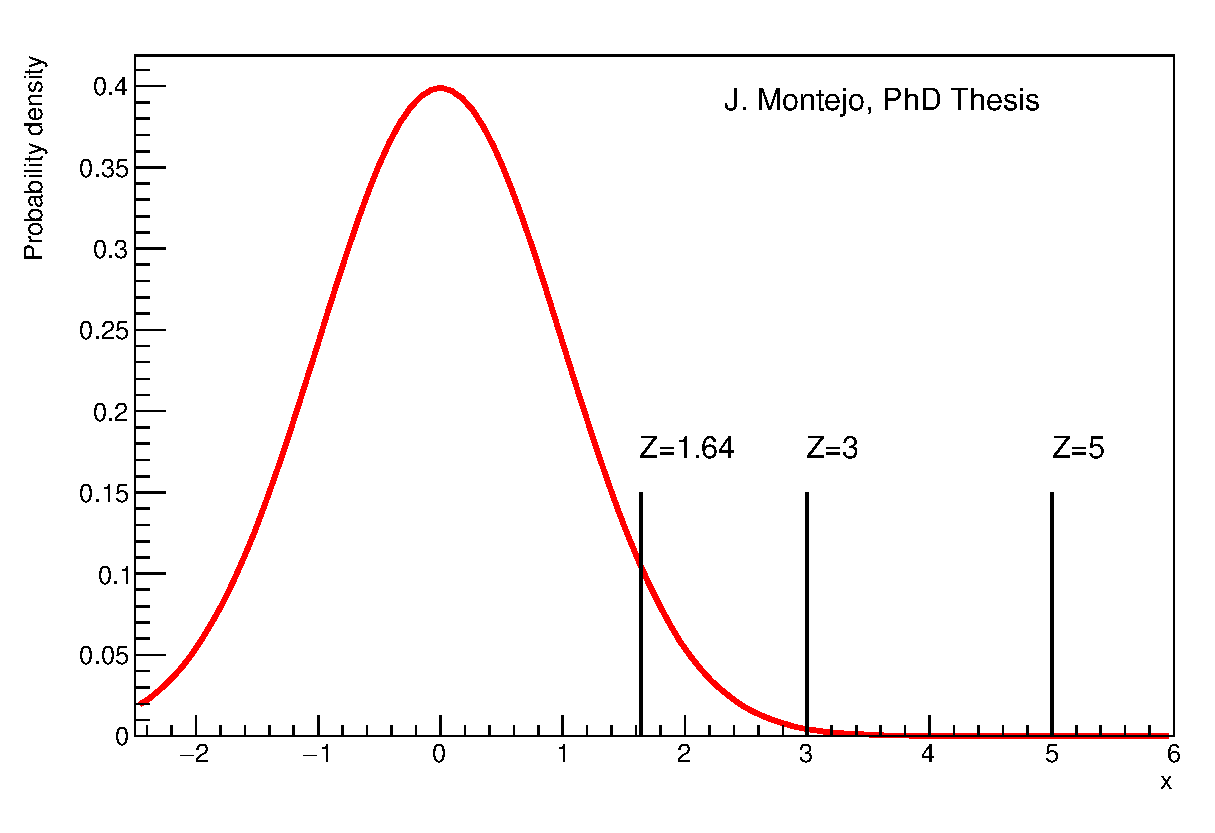
\includegraphics[width=0.65\textwidth]{Statistics/Figures/significance}
      \caption{Thresholds that have been chosen as convention to claim the exclusion of a new physics process (Z=1.64), evidence for new physics (Z=3) and discovery (Z=5).}
      \label{fig:significance}
    \end{figure}

   \subsection{$CL_s$ method}
   \label{subsection:CLs_method}
   The $p_\mu$ value extracted from the observed data is subject to statistical fluctuations and it can lead to unphysical exclusions when a downward fluctuation in the observed number events occur.
   In order to avoid exclusions of $\mu$ values that the search is a priori not sensitive to, the $CL_s$ method~\cite{CLs} is introduced.
   The $CL_s$ value is defined as a ratio of probabilities:
   \begin{equation}
     \label{eq:CLS}
     CL_s=\frac{p_\mu}{1-p_0} %=\frac{p_{s+b}}{1-p_b}
   \end{equation}
   where $p_{\mu}$ and $p_0$ quantify the compatibilities between the data and the signal-plus-background and 
   background-only hypotheses, respectively. 
    A downward background fluctuation in data will lead to small values of $1-p_0$, increasing
    the $CL_s$ value and avoiding the exclusion of too small \xsecs. 
   For searches at the LHC, the $CL_s$ value is used instead of $p_\mu$ to set upper limits.
   If $CL_s < 0.05$, the signal-plus-background hypothesis with a signal strength $\mu$ is excluded at \unit[95]{\%} confidence level.
    
   \section{Likelihood function and profile likelihood ratio}
   The likelihood function gives the probability of an observation to have been originated by a given model. Considering the minimum division in which the observed data is classified, i.e. one single histogram bin in one region, the expected number of events in the bin $i$ can be written as:

    \begin{equation}
      \label{eq:expectation_bin}
      E_i = \mu \cdot s_i + b_i,
    \end{equation}
    where $s_i$ and $b_i$ correspond to the number of expected signal and background events, respectively, in the $i$-th bin.
    This expectation has to be compared to the observation of $n_i$ events in data. Assuming that the data follows a Poisson distribution, the likelihood for the observed data to be produced by the model is:
    \begin{equation}
      \label{eq:likelihood_bin}
      L_i(\mu)=\frac{(\mu s_i+b_i)^{n_i}}{n_i !}e^{-(\mu s_i+b_i)}.
    \end{equation}

    The prediction of the model however, is affected by uncertainties in the form of systematic and statistical errors. The effect of these uncertainties on the predictions can be modeled through nuisance parameters (NP), $\theta$. A variation in the NP produces a change in the expected number of events, $s_i(\theta)$ and $b_i(\theta)$, therefore the maximization of the likelihood leads to adjustments in the NP in order to improve the agreement of the expectation with the observed data. 
    The NP are characterized by a pdf $\rho(\theta)$, encoding the information about its best estimate and width, which is related to the size of the uncertainty. The pdfs for each systematic uncertainty are determined beforehand by auxiliary measurements. The pdf is also included in the likelihood and is usually referred to as \textit{penalty term} or \textit{prior} on $\theta$. Depending on the NP, different functional forms can be assumed for the pdf:
    \begin{itemize}
      %%%%%%%%% Gaussian distribution
    \item A Gaussian pdf is the common assumption for most systematic uncertainties. 
      Systematic uncertainties that change the shape of the final discriminant are assumed to have a Gaussian prior:
      \begin{equation}
        \label{eq:NPGaus}
        \rho (\theta)= \frac{1}{\sqrt{2\pi}\sigma}\exp\left(-\frac{(\theta-\hat{\theta})^2}{2\sigma^2}\right).
      \end{equation}
      For example, the jet energy scale is defined by its measured value, $\hat{\theta}_{\mathrm{JES}}$, and an uncertainty, $\sigma_{\mathrm{JES}}$. The variation of $\theta_{\mathrm{JES}}$ may improve the data/MC agreement and therefore increase the Poisson term in the likelihood maximization, but large departures from its nominal value are penalized through $\rho (\theta_{\mathrm{JES}})$.
      %This pdf is not suitable for positively defined observables.
      %%%%%%%%%Log-normal distribution
    \item The log-normal pdf is used for normalization uncertainties, given its property that the effect on the estimation is bounded to positive values:
      \begin{equation}
        \label{eq:NPLogNormal}
        \rho (\theta) = \frac{1}{\sqrt{2\pi}\ln (\sigma)}\exp \left(- \frac{(\ln(\theta/\hat{\theta}))^2}{2(\ln(\sigma))^2}\right)\frac{1}{\theta}.
      \end{equation}
      The parameter $\sigma $ characterizes the width of the log-normal distribution.
      %%%%%%%%%Gamma distribution 
    \item The Gamma pdf is used to describe statistical uncertainties associated with the number of 
      selected MC events. The event rate $n$ in a certain region is related to the number
      of events N in MC using the relation $n=\alpha\cdot N$. The gamma distribution, as a function of these 
      variables, is expressed as follow:
      \begin{equation}
        \label{eq:NPGamma}
        \rho (n) = \frac{1}{\alpha}\frac{(n/\alpha)^N}{N!}e^{\left(-n/\alpha \right)}.
      \end{equation}
    \end{itemize}
    An example of the different pdfs for several values of the relative uncertainty is given in figure~\ref{fig:pdf}. In the limit of small uncertainties the log-normal and Gamma pdfs approximate to a Gaussian distribution.
\begin{figure}[!t]
  \begin{center}
    \begin{subfigure}{0.49\textwidth}
        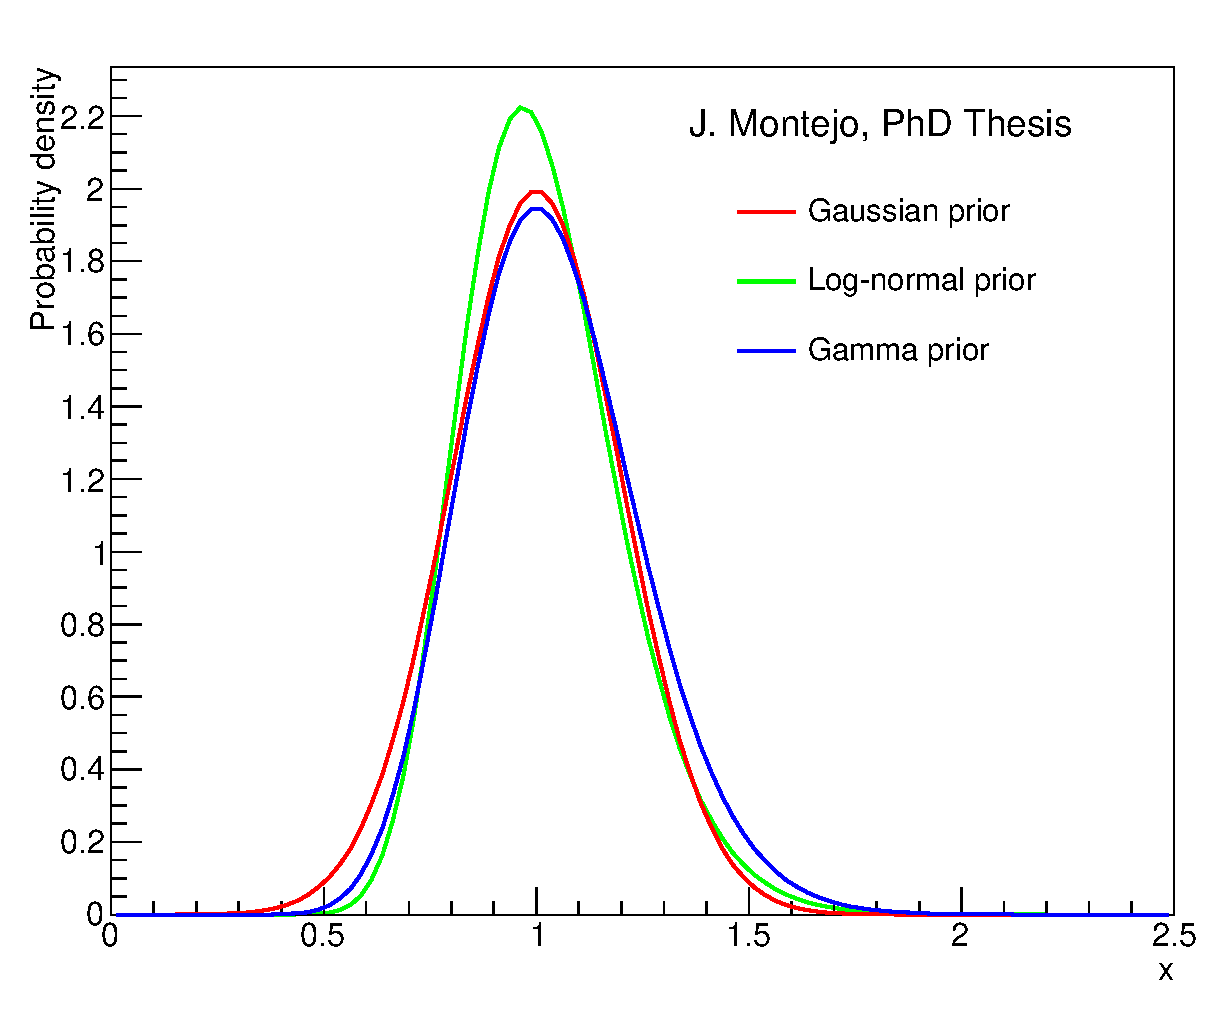
\includegraphics[width=\textwidth]{Statistics/Figures/prior0_20.eps} 
        \caption{}
      \end{subfigure}
    \begin{subfigure}{0.49\textwidth}
        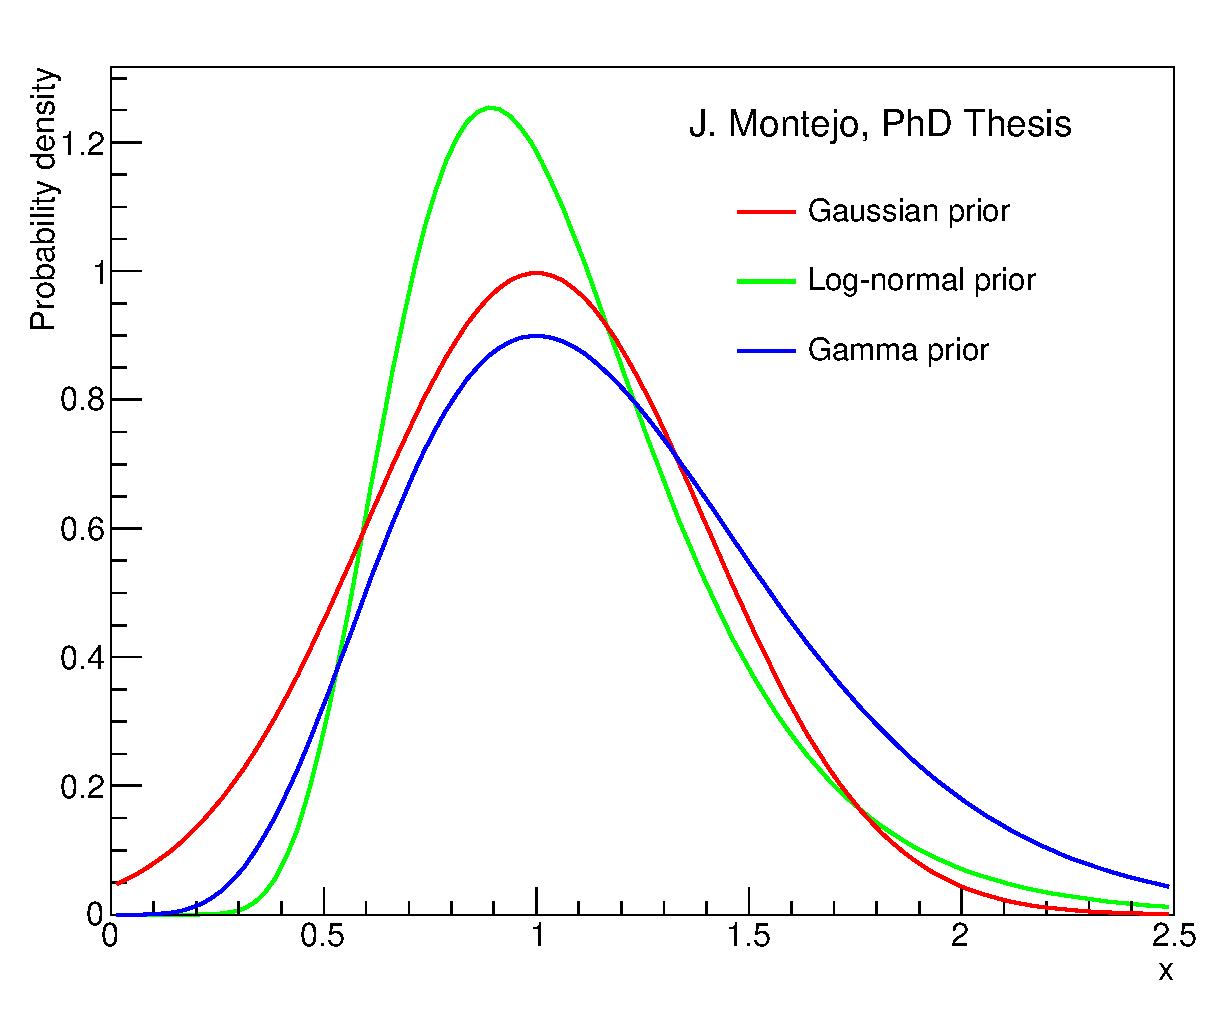
\includegraphics[width=\textwidth]{Statistics/Figures/prior0_40.eps}
        \caption{}
      \end{subfigure}
  \end{center}
  \caption{Illustration of different pdfs for a normalized variable x with mean $\hat{x}=1$ and different values of the relative uncertainty: 
(a) 0.2 and (b) 0.4.
}
  \label{fig:pdf}
\end{figure}

    This description of the priors is based on the absolute values of the NP and their uncertainties, and understanding the fit result becomes very difficult since it requires the knowledge of the pre-fit values for each NP.
    In order to simplify the analysis, all NP are redefined in order to be centered at zero and with a width of one. In the case of a Gaussian NP this is equivalent to: 
    \begin{equation}
      \theta' = \frac{\theta-\hat{\theta}}{\sigma}~.
      \label{eq:np_redefinition}
    \end{equation}
    In this way, the fitted NP can be easily compared with the pre-fit values. 
    A fitted value close to 0 and a fitted error close to 1 indicates that the
    data did not have enough statistical power to induce a pull in the nuisance parameter and reduce the original uncertainty.
    Fitted values away from 0 indicate that the modified MC is in better agreement with the observed data. 
    Reduced errors indicate that the assigned prior was too large, and the observed data allows reducing the allowed range for the systematic variation.

    %After the redefinition, the effect of the NP on the background can be modelled as:
    %\begin{equation}
    %  b_i(\theta) = b_i^0(1+\sum_k\theta_k\Delta b_k)~,
    %  \label{eq:np_effect}
    %\end{equation}
    %where $\Delta b_k$ is the variation produced on the background from a shift of one standard deviation of $\theta_k$.

    Finally, the full likelihood can be written as:
    \begin{equation}
      \label{eq:likelihood}
      L(\mu,\theta)=\prod_{i=1}^{N}\frac{(\mu s_i+b_i)^{n_i}}{n_i !}e^{-(\mu s_i+b_i)} \prod_{k=1}^{M}\rho(\theta_k)~.
    \end{equation}

    The likelihood function can be globally maximized, where both the signal strength and the nuisance parameters are fitted. This unconditional maximum likelihood is denoted by $L(\hat{\mu},\hat{\theta})$. The likelihood can also be maximized for a fixed value of $\mu$, and the resulting conditional maximum likelihood is denoted by $L(\mu,\hat{\hat{\theta}}(\mu))$.     
    The ratio of both defines the profile likelihood ratio which is the test statistic of choice for most searches at the LHC, including the analyses described in this dissertation:
    \begin{equation}
      \label{eq:profileL}
      \lambda(\mu)=\frac{L(\mu,\hat{\hat{\theta}}(\mu))}{L(\hat{\mu},\hat{\theta})}.
    \end{equation}

    The profile likelihood ranges from $0<\lambda<1$, with values of $\lambda$ close to one implying good agreement between the data and the hypothesized value of $\mu$. 
    A more common form for the test statistic is $q_\mu = -2 \ln \lambda (\mu)$.

   \subsection{$p$-values}
   \label{subsection:pvalues}
   From the test statistic a $p$-value can be computed, giving the probability that the observed data originates from the considered hypothesis:
   
    \begin{equation}
      \label{eq:pmu}
      p_\mu= \int^\infty_{q_{\mu , {\rm obs}}}f(q_\mu|\mu)~dq_\mu.
    \end{equation}
    where ${q_{\mu , {\rm obs}}}$ is the observed value of the test statistic in data and $f(q_\mu|\mu)$ denotes
    the pdf of $q_\mu$ assuming the hypothesis $\mu$. 
    The computation of background-only quantities such as $p_0$ are just special cases with $\mu=0$ and will not be defined separately in the following.
    
    In general, the pdf $f(q_\mu|\mu')$ with $\mu \neq \mu'$ is also needed in order to test the compatibility of an hypothesis $\mu$ when the data is originated from a model with $\mu'$. This ``off-diagonal'' hypothesis testing is useful to characterize the expected performance of an analysis. The median significance for a discovery is computed using $f(q_0|1)$, whereas the expected \unit[95]{\%} CL in the absence of a signal is computed from $f(q_{1}|0)$.
    An illustration on how the expected $p_0$ is obtained is given in figure~\ref{fig:p0exp}.
%    The procedure to obtain the pdf $f(q_\mu|\mu')$ is explained in section~\ref{subsec:asimov}.

    \begin{figure}[t!]
      \begin{center}
        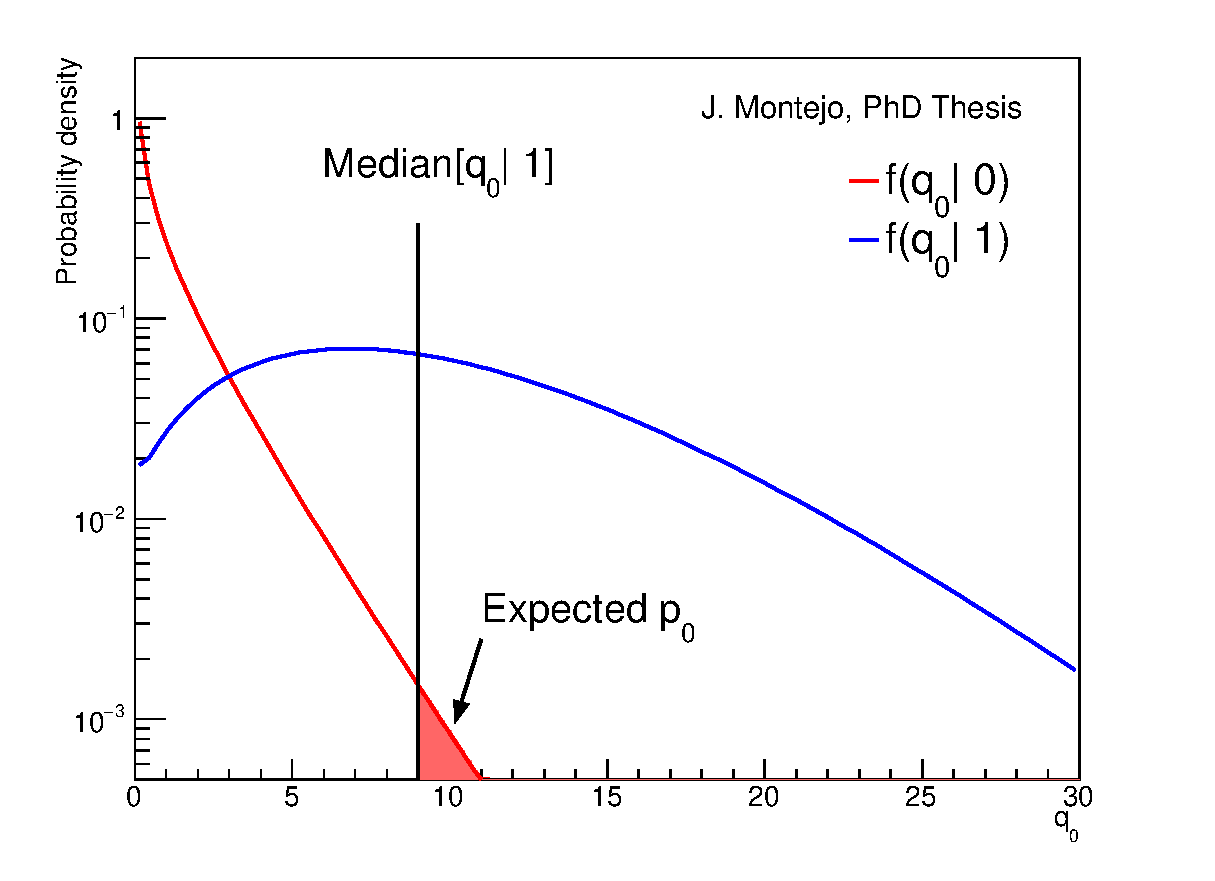
\includegraphics[width=.7\textwidth]{Statistics/Figures/pvalue_0_1_hist0.eps}
        \caption{
          The distribution of the statistic $q_0$ under the hypotheses of signal-plus-background and
          background-only. The shaded area corresponds to the median $p_0$ that would be obtained if the background-only hypothesis is tested on a dataset originating from a signal-plus-background model.
          \label{fig:p0exp}}
      \end{center}
    \end{figure}

    \subsection{Approximate distributions for the test statistic}
    \label{subsec:asimov}
    
    The computation of a $p$-value associated with a hypothesis requires the full distribution of the test statistic as shown in equation~\ref{eq:pmu}. 
    The estimation of the $q_\mu$ distribution can be done with MC methods, but these
    methods are computationally expensive. For a discovery 
    with $p_0\sim 10^{-7}$, about $10^8$ pseudo-experiments have to be simulated. 

    In the limit of large statistics or ``asymptotic limit'', an approximation can be introduced to describe the profile likelihood ratio~\cite{Cowan:2010js}.
    If data is assumed to be distributed according to a strength parameter $\mu'$, then Wald's approximation~\cite{WaldApprox}
    can be used to write:
    \begin{equation}
      \label{eq:AsymAprox}
      q_\mu = -2\ln \lambda(\mu) = \frac{(\mu-\hat{\mu})^2}{\sigma^2} + \mathcal{O}(1/\sqrt{N}),
    \end{equation}
    where the fitted strength parameter $\hat{\mu}$ follows a Gaussian distribution with a mean $\mu'$ and standard deviation $\sigma$, and $N$
    accounts for the data sample size. 
    The value of $\sigma$ is estimated from an artificial 
    data set known as ``Asimov data set''~\cite{Cowan:2010js}.
    The Asimov data set is defined as the one where the pseudo-data is equal to the expectation value, i.e. to the sum of background predictions.
    %To construct it, the pseudo-data is forced to be equal
    %to its expectation value $n_{i,A} = E[n_i]=\mu's_i(\theta)+b_i(\theta)$ and all NPs are set to the 
    %values obtained from the best fit to data.

    Using equation~\ref{eq:AsymAprox} and neglecting the term $\mathcal{O}(1/\sqrt{N})$, the pdf for the test statistic $q_\mu$ follows 
    a noncentral chi-square distribution with one degree of freedom:
    \begin{equation}
      f(q_\mu, \Lambda) = \frac{1}{2\sqrt{q_\mu}}\frac{1}{\sqrt{2\pi}}\left[
        \exp\left(-\frac{1}{2}(\sqrt{q_\mu}+\sqrt{\Lambda})^2\right) +
        \exp\left(-\frac{1}{2}(\sqrt{q_\mu}-\sqrt{\Lambda})^2\right) \right] ,
      \label{eq:qmu_pdf}
    \end{equation}
    where the noncentrality parameter $\Lambda$ is: 
    \begin{equation}
    \Lambda=\frac{(\mu-\hat{\mu})^2}{\sigma^2}.
      \label{eq:Lambda}
    \end{equation}
    
    \begin{figure}[tb!]
      \begin{center}
        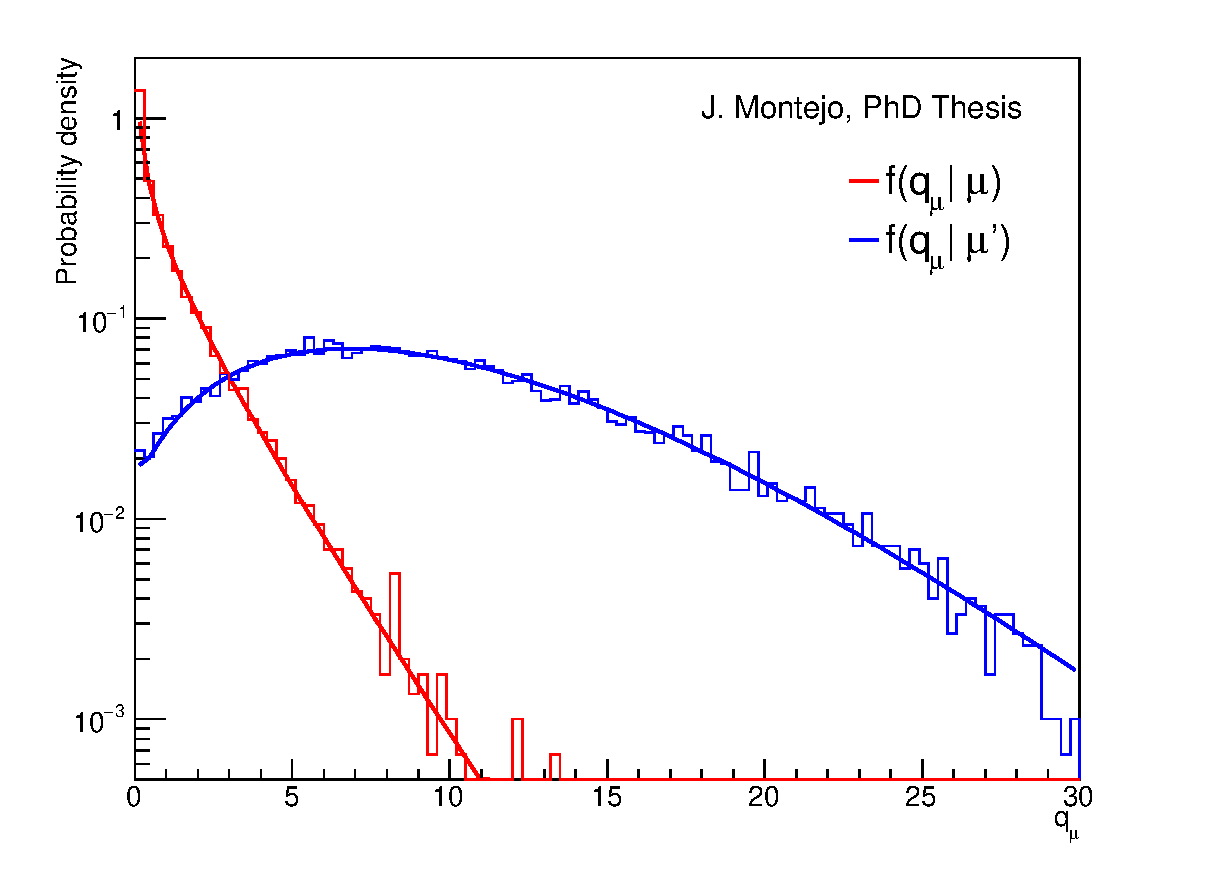
\includegraphics[width=.7\textwidth]{Statistics/Figures/pvalue_mu_muprime_hist1.eps}
        \caption{
          The distribution of the statistic $q_\mu$ under two hypotheses, one of them with $\mu' \neq \mu$. 
          MC predictions are given by the histograms and solid curves are obtained from the asymptotic approximation.
          \label{fig:asimov}}
      \end{center}
    \end{figure}

    An example of distributions obtained with this method is shown in figure~\ref{fig:asimov}
    where the histograms are from MC and the solid curves are the predictions of the asymptotic approximation.
    For the searches described in this dissertation the asymptotic approximation is used in order to compute the relevant $p$-values.

   \subsection{Profiling in action}
   One the main benefits from the profiled likelihood approach is that the fit to data can provide additional information on the systematic uncertainties obtained from external inputs. The NP can be pulled to maximize the agreement of the background prediction with data, and the uncertainty on the NP can be reduced with respect to its initial value. This reduction in the uncertainty can significantly improve the sensitivity of the analysis.

   The reduction of the uncertainty, also referred to as profiling or constraining, occurs when large effects of a particular systematic uncertainty are not compatible with the range allowed by the data statistics. This reduction of the uncertainty produces an improvement in the analysis sensitivity, but some caution is needed as to not introduce overconstrains due to a too simplistic systematic treatment.
   When several NP have a similar effect, the total variation might be larger than the precision allowed in data. Since their effect can not be disentangled the individual NPs are not constrained but a correlation (or anti-correlation) is established such that the combined effect is at the level of the data statistics. 

   In other cases the effect of a systematic is much smaller than the statistical error on the data, either because the effect of the systematic uncertainty is very small or because it affects a region of phase space where there is very little data. In this situation the constraint term in the likelihood drives the NP to stay at a value of zero and its error is the same as the given input uncertainty. 

   The fitting procedure is best illustrated with an example based on toy data. Let us consider an analysis with two regions, denoted A and B. For simplicity, we will assume that each region contains only one background, which will we named also A and B. The MC prediction is 80 and 100 events respectively in each channel, and the data observation is 100 events per channel. This setup is shown in figure~\ref{fig:toy_prefit}.
   \begin{figure}[tb!]
     \centering
     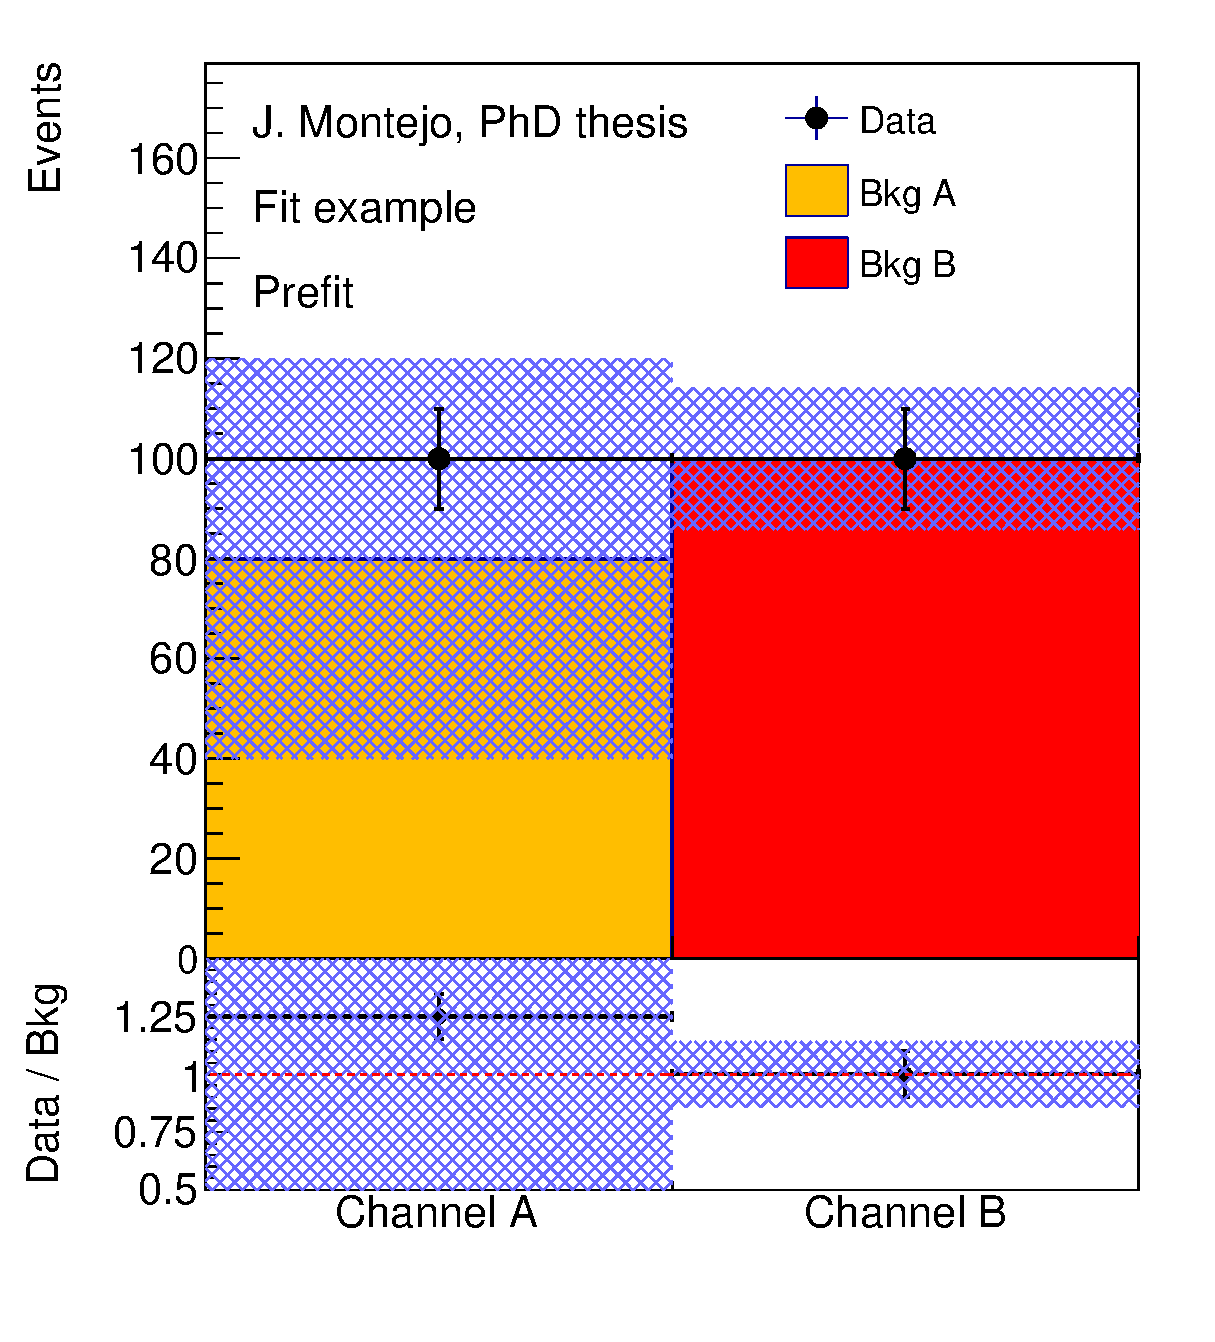
\includegraphics[width=0.6\textwidth]{Statistics/Figures/fitexample/hist_AB_prefit.eps}
     \caption{Setup of the toy data and MC used to exemplify the profiled likelihood fit. The MC prediction and uncertainty is shown before the fit. }
     \label{fig:toy_prefit}
   \end{figure}

   The following systematic uncertainties are implemented:
   \begin{itemize}
     \item A \unit[50]{\%} normalization uncertainty on the background A, referred to as ``Normalization A''.
     \item Two normalization uncertainties with a value of \unit[10]{\%} on the background B, referred to as ``Normalization B1'' and ``Normalization B2'' respectively.
     \item A luminosity uncertainty of \unit[1]{\%}, affecting both backgrounds.
   \end{itemize}

   A profile likelihood fit is performed to the toy data, and the result of the fit is shown in figure~\ref{fig:toy_result}. The deficit of 20 events in the region A is corrected by pulling the nuisance parameter for the normalization of background A by 0.5.\footnote{The exact value is not 0.5, although this would bring the MC prediction to 100 events, but slightly below since the penalty term in the likelihood penalizes slightly the pull away from zero. } 
   This results in an increase of \unit[25]{\%} of the background that corrects the disagreement. In the region B no pull is introduced given the pre-fit agreement between toy data and prediction.

   \begin{figure}[tb!]
     \centering
     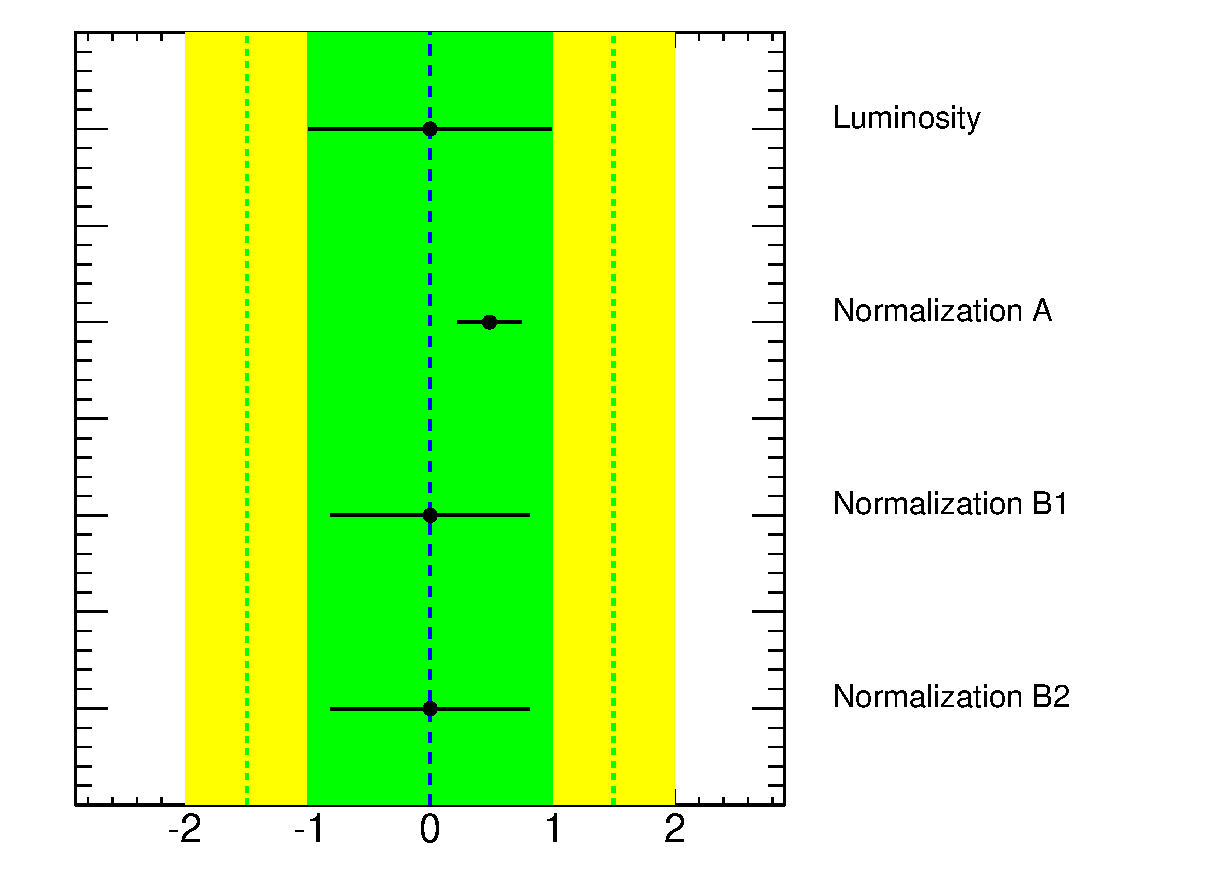
\includegraphics[valign=t, width=0.52\textwidth]{Statistics/Figures/fitexample/toyFit.eps}
     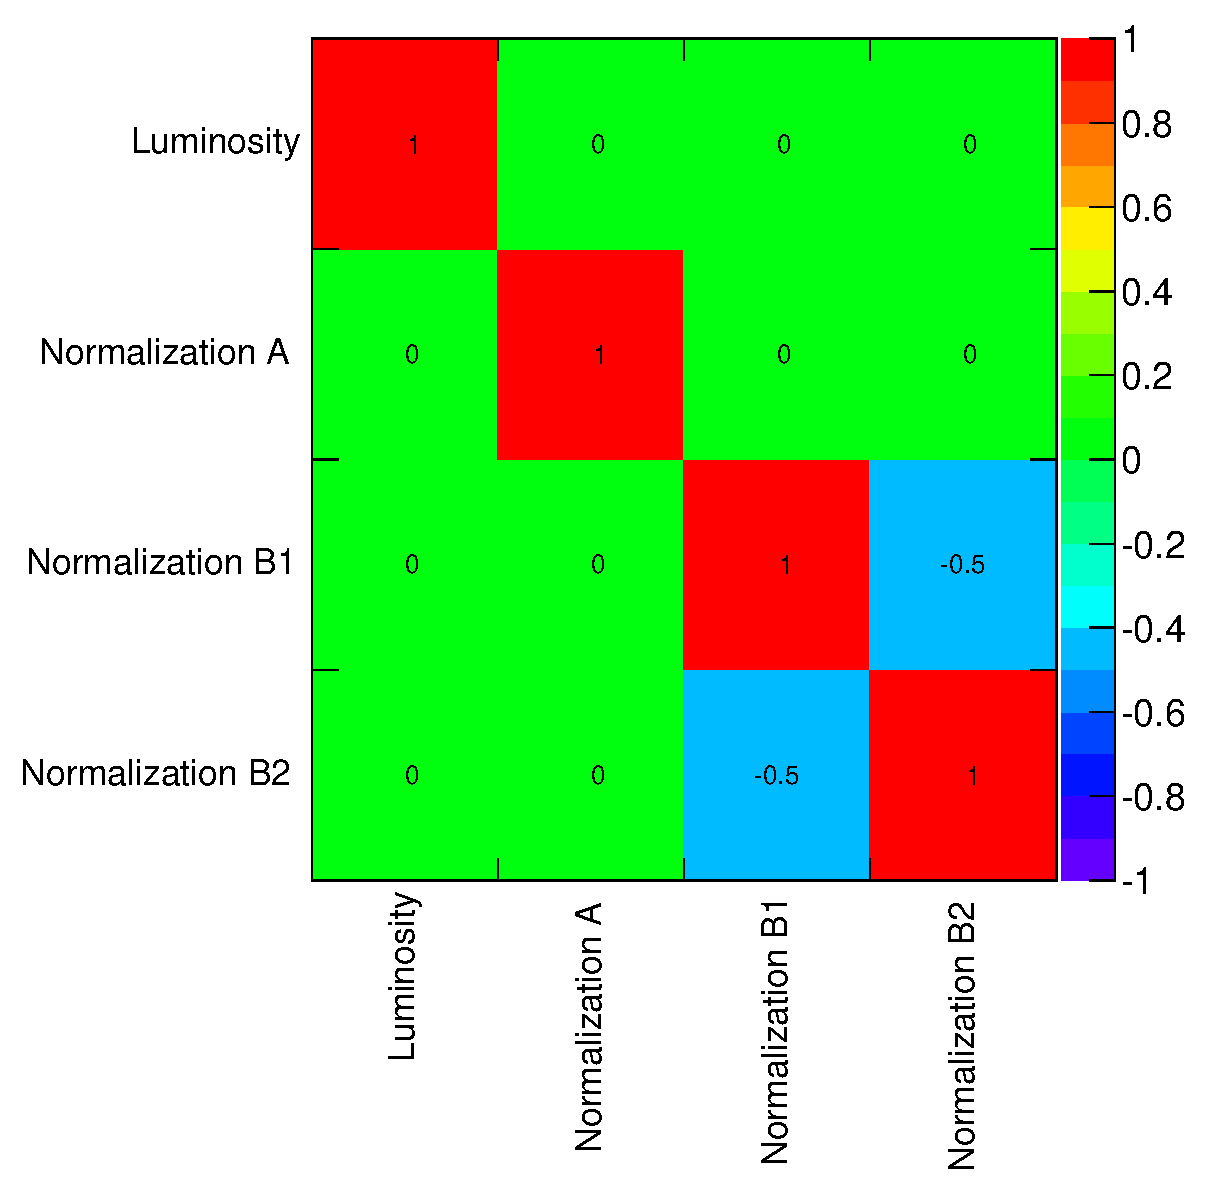
\includegraphics[valign=t, width=0.47\textwidth]{Statistics/Figures/fitexample/toyCorr.eps}
     \caption{Fitted nuisance parameters (left) and correlation matrix (right) after the fit to the toy data. }
     \label{fig:toy_result}
   \end{figure}

   With 100 events in the toy data, the relative precision that can be achieved in the normalization is \unit[10]{\%}. The systematic uncertainty that is assigned for background A is much larger, and the fit to data can reduce the uncertainty to 0.25 times the pre-fit value.\footnote{The pre-fit values are always used as reference, giving a post-fit uncertainty of \unit[12.5]{\%}, equivalent to 10 events. Notice that this is equal to an uncertainty of \unit[10]{\%} respect to the corrected MC.} This reduction in the uncertainty allows a better sensitivity for any signal that could be present in region A.

   The situation in region B is a bit different given that there are two degenerate uncertainties. Focusing on one of them, the prior uncertainty of \unit[10]{\%} is slightly constrained. The likelihood at the $\pm 1\sigma$ points is penalized by both the prior and the Poisson term. This can also be understood in the following way: if this region would have been included in the measurement providing the prior for the systematic, the error on the nuisance parameter prior would be reduced.
   Given that two systematic uncertainties are present, their combined effect, if assumed uncorrelated, would exceed the \unit[10]{\%} precision in data. The fit develops an anti-correlation among them of $\rho = \unit[-50]{\%}$ so that the combined effect is:
   \begin{equation}
     \begin{split}
       \sigma_{B1} &= \sigma_{B2} = \sigma \\
       \sigma_{B1 \otimes B2} &= \sqrt{\sigma_{B1}^2+\sigma_{B2}^2+2\sigma_{B1}\sigma_{B2}\rho} = \sigma~.
     \end{split}
   \end{equation}
  Through the anti-correlation the post-fit uncertainty is reduced to the level of the data statistics.
  Finally, the luminosity uncertainty has a very small effect compared to the data precision. Therefore the final result of the nuisance parameter is dominated by the prior and kept at $\theta_{\rm Luminosity}=0\pm 1$.

  Figure~\ref{fig:toy_postfit} shows the toy data and MC after the fit. The MC prediction has been corrected and the systematic uncertainties are constrained as discussed.
   \begin{figure}[tb!]
     \centering
     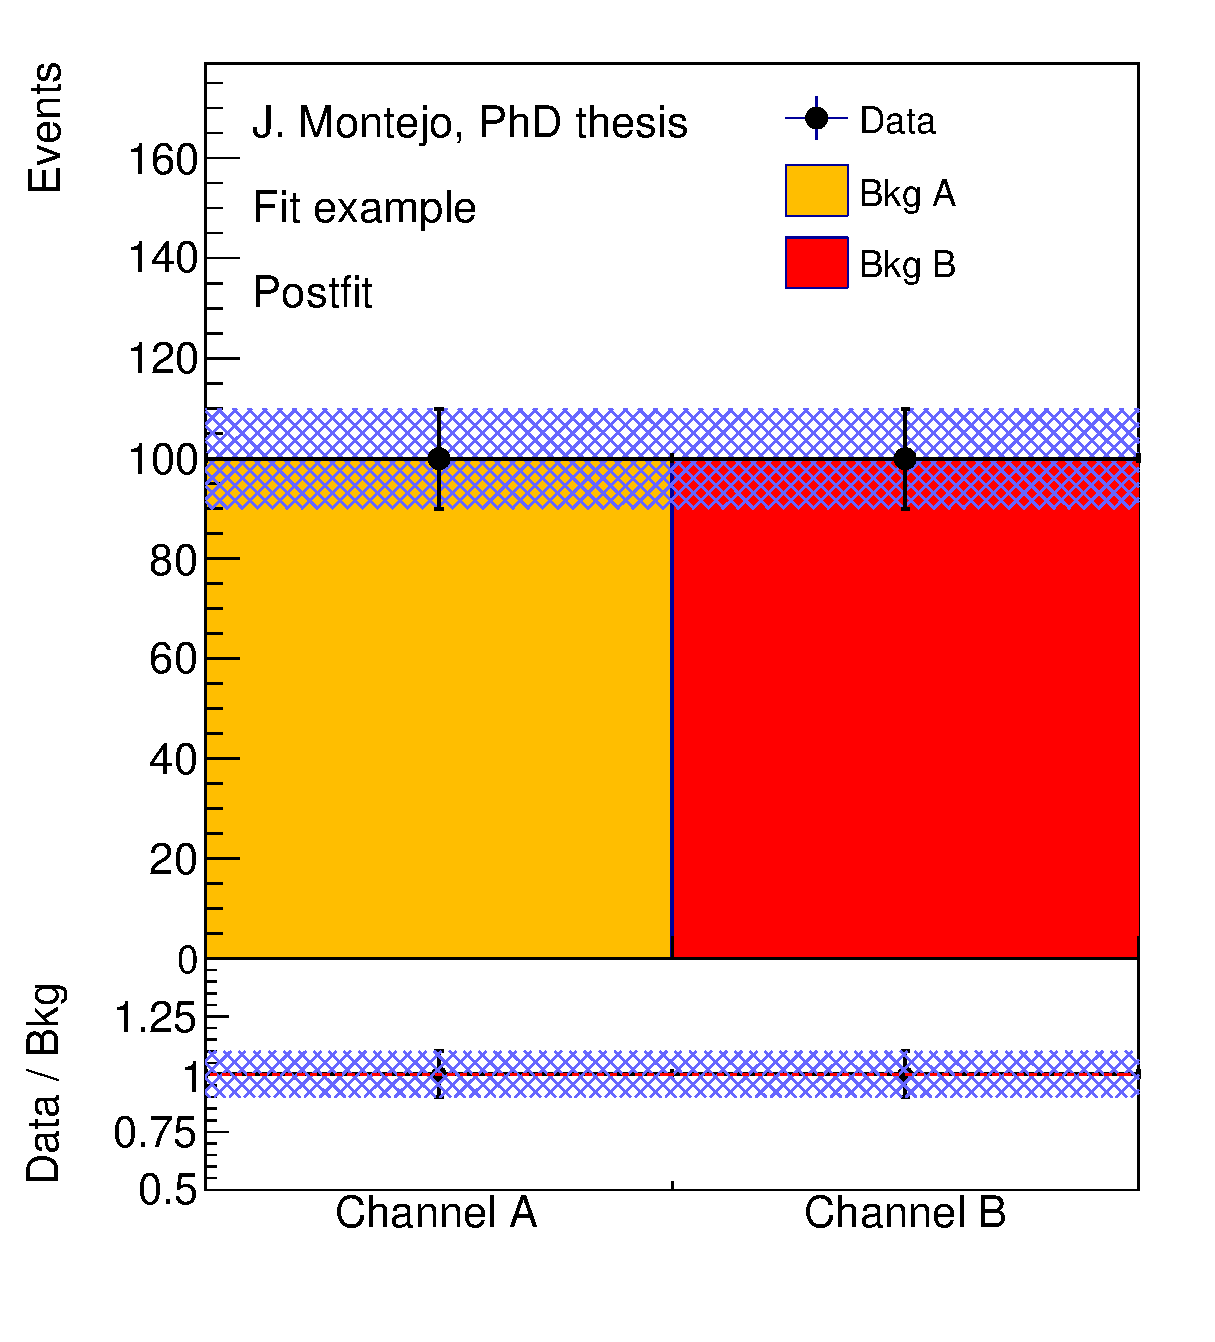
\includegraphics[width=0.6\textwidth]{Statistics/Figures/fitexample/hist_AB_postfit.eps}
     \caption{Setup of the toy data and MC used to exemplify the profiled likelihood fit. The MC prediction and uncertainty is shown after the fit. }
     \label{fig:toy_postfit}
   \end{figure}
   
  A background-only scenario has been discussed up until now. Let us include a signal process that contributes with 20 events to region A, the exact amount needed to fill the deficit between toy data and prediction.

  The fit result with the inclusion of a signal process is shown in figure~\ref{fig:toy_resultSB}. Region B is unaffected but there are two main changes in region A: the normalization of background A is no longer pulled since the agreement is perfect, and the constrain on the systematic uncertainty disappears completely. The signal strength and the normalization of background A are completely degenerate, and the variation of the signal strength in any direction can be compensated by a change in the background. Since the signal has no penalty term, the allowed variation is determined by the background uncertainty. A \unit[50]{\%} variation in the background, or 40 events, translates into a \unit[200]{\%} uncertainty on the signal, which also amounts to 40 events.
   \begin{figure}[tb!]
     \centering
     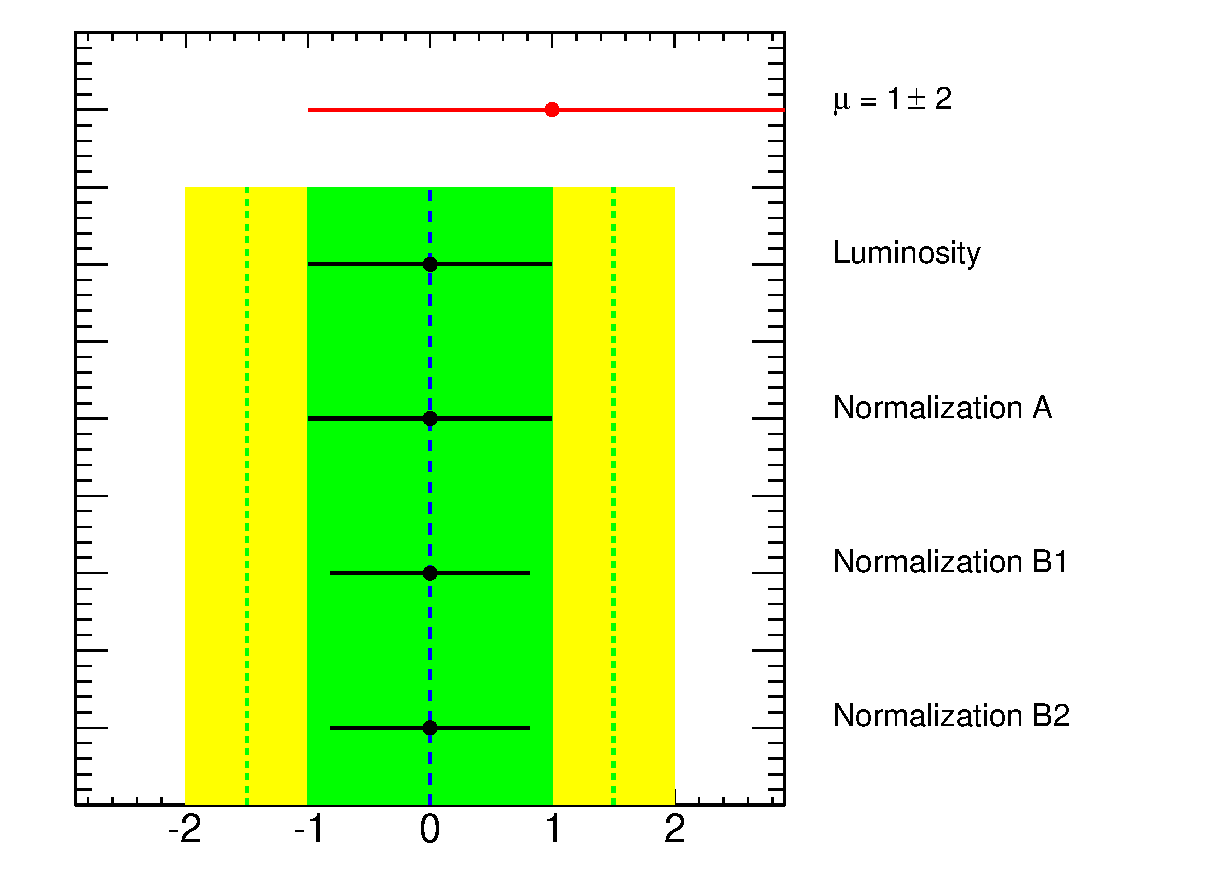
\includegraphics[valign=t, width=0.52\textwidth]{Statistics/Figures/fitexample/toyFitSB.eps}
     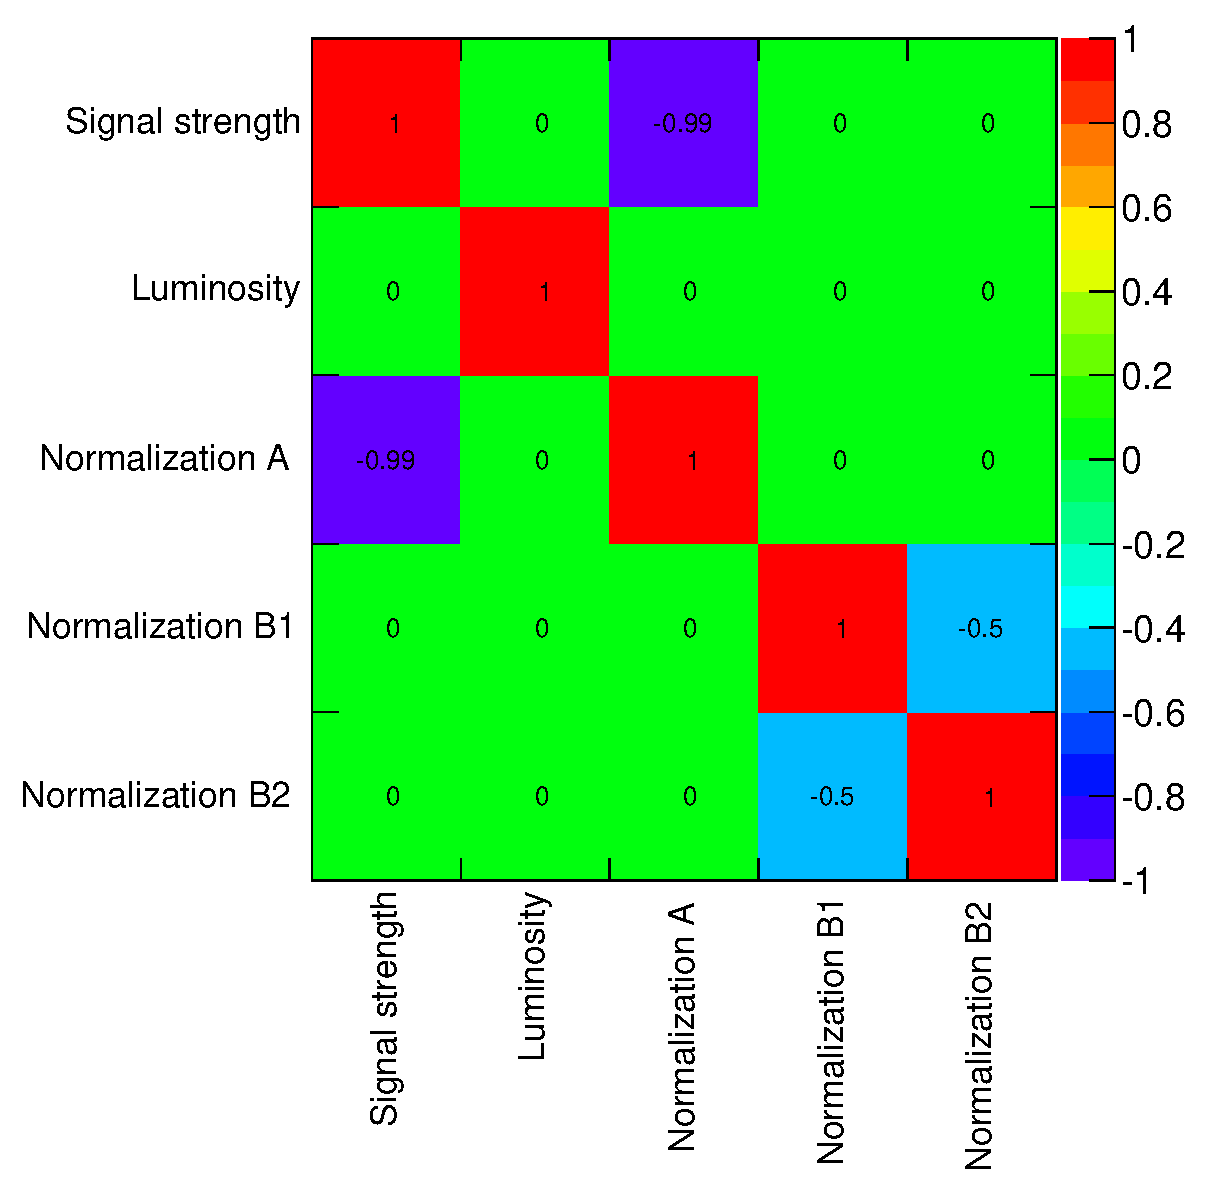
\includegraphics[valign=t, width=0.47\textwidth]{Statistics/Figures/fitexample/toyCorrSB.eps}
     \caption{Fitted nuisance parameters (left) and correlation matrix (right) after the fit to the toy data under the signal-plus-background hypothesis. }
     \label{fig:toy_resultSB}
   \end{figure}

  In this situation it seems obvious that the systematic uncertainty that will degrade the sensitivity of the analysis is the normalization of background A. This can be quantified through the NP \textit{ranking} procedure. 
  The effect of a NP on $\mu$ is calculated by fixing the corresponding
  nuisance parameter at $\hat{\rm{\theta}} \pm \sigma_{\rm{\theta}}$, where
  $\hat{\rm{\theta}}$ is the fitted value of the nuisance parameter and
  $\sigma_{\rm{\theta}}$ is its post-fit uncertainty, and
  performing the fit again. The difference between the default and the modified $\mu$, $\Delta\mu$,
  represents the effect on the signal of this particular systematic uncertainty.
  The same procedure can also be performed before the fit to data in order to evaluate the gain introduced
  by the constraints.
Figure~\ref{fig:toy_ranking} shows the ranking of the NP, demonstrating the effect of various systematic uncertainties on
the fitted value of $\mu$ and the constraints provided by the toy data. In this simple example only one NP is relevant, and the pre-fit and post-fit impacts on the signal strength are the same. 

The ranking of NPs is a very powerful tool and will be used to identify the leading systematic uncertainties affecting the sensitivity of the search, so that they can be studied in more detail.
   \begin{figure}[tb!]
     \centering
     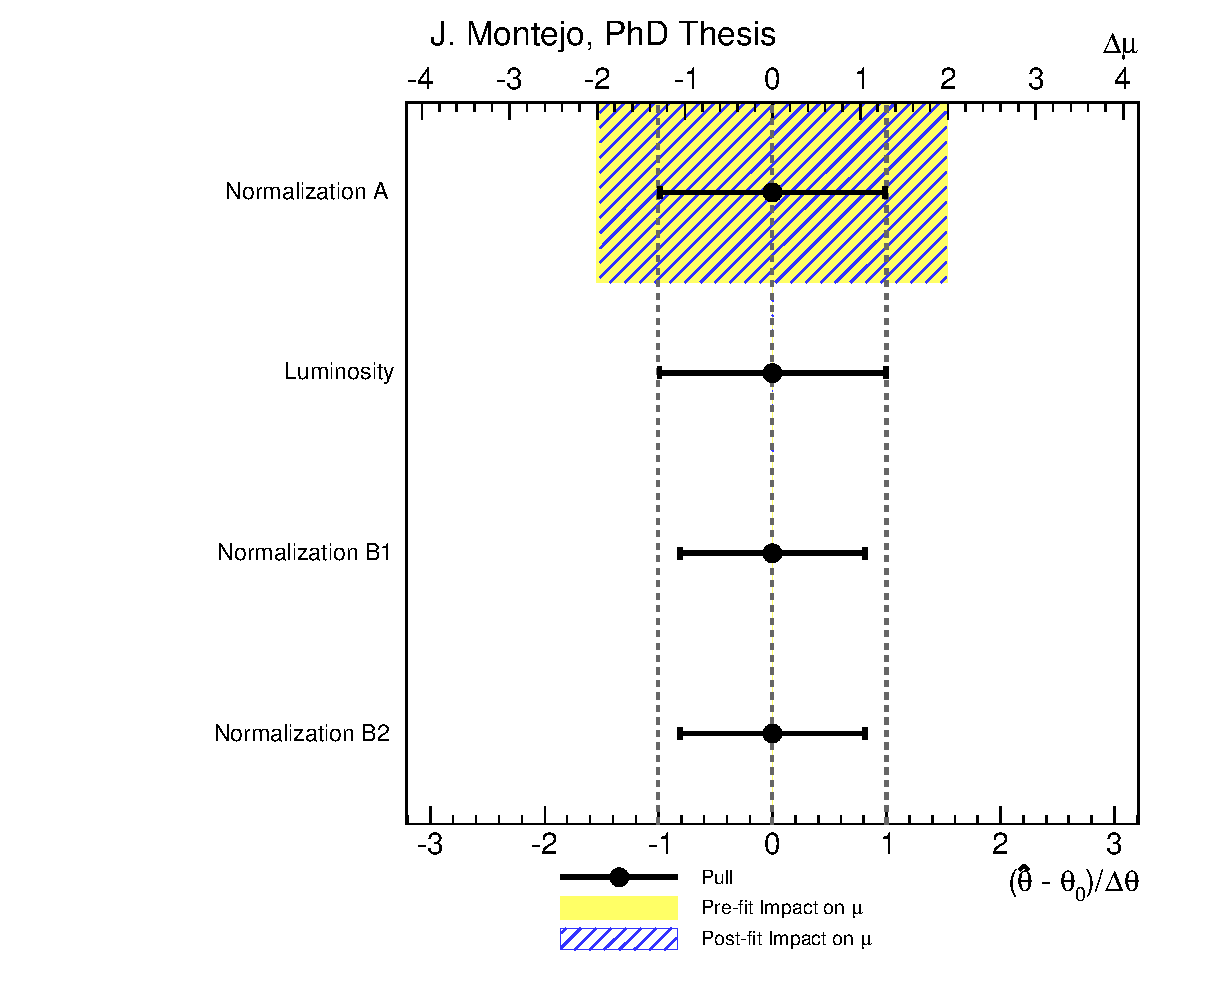
\includegraphics[width=0.8\textwidth]{Statistics/Figures/fitexample/toy_pulls_125.eps}
     \caption{
     Ranking of nuisance parameters according to their impact on the measured signal strength. 
The points, which are drawn conforming to the scale of the bottom axis, show the 
deviation of each of the fitted nuisance parameters, $\hat{\rm{\theta}}$, from 
$\rm{\theta_{0}}$, which is the nominal value of that nuisance parameter, in units 
of the pre-fit standard deviation $\Delta\theta$. The error bars show the 
post-fit uncertainties, $\sigma_{\theta}$.
The nuisance parameters are 
sorted according to the post-fit effect of each on $\mu$ (hashed blue 
area) conforming to the 
scale of the top axis, with those with the largest impact at the top. 
   }
     \label{fig:toy_ranking}
   \end{figure}

\clearpage
\bibliographystyle{Bibliography/atlasnote}
\bibliography{Bibliography/myBib}
